\section{Energy and Flavor Separation By Time-of-Arrival}
\label{mechanism}

The power of this technique stems from the fact that, in contrast to
off-axis measurements, the different neutrino energy spectra can be
selected within the same detector. Moreover, these timing
relationships can be applied in near and far detector alike. 

We emphasize that the time of individual neutrino events is determined
by the position of the vertex with respect to the phase of the RF, and
requires no time measurement capability in the detector
itself. Instead, the RF
structure is measured bunch-by-bunch by a 10-15 GHz waveform sampling
system by the muon monitor system (MMS). The recorded stream of bunch 
structure parameters or profiles is time-stamped and synchronized with
the detector data as a separate operation.

\begin{figure}[t]
	\begin{center}
        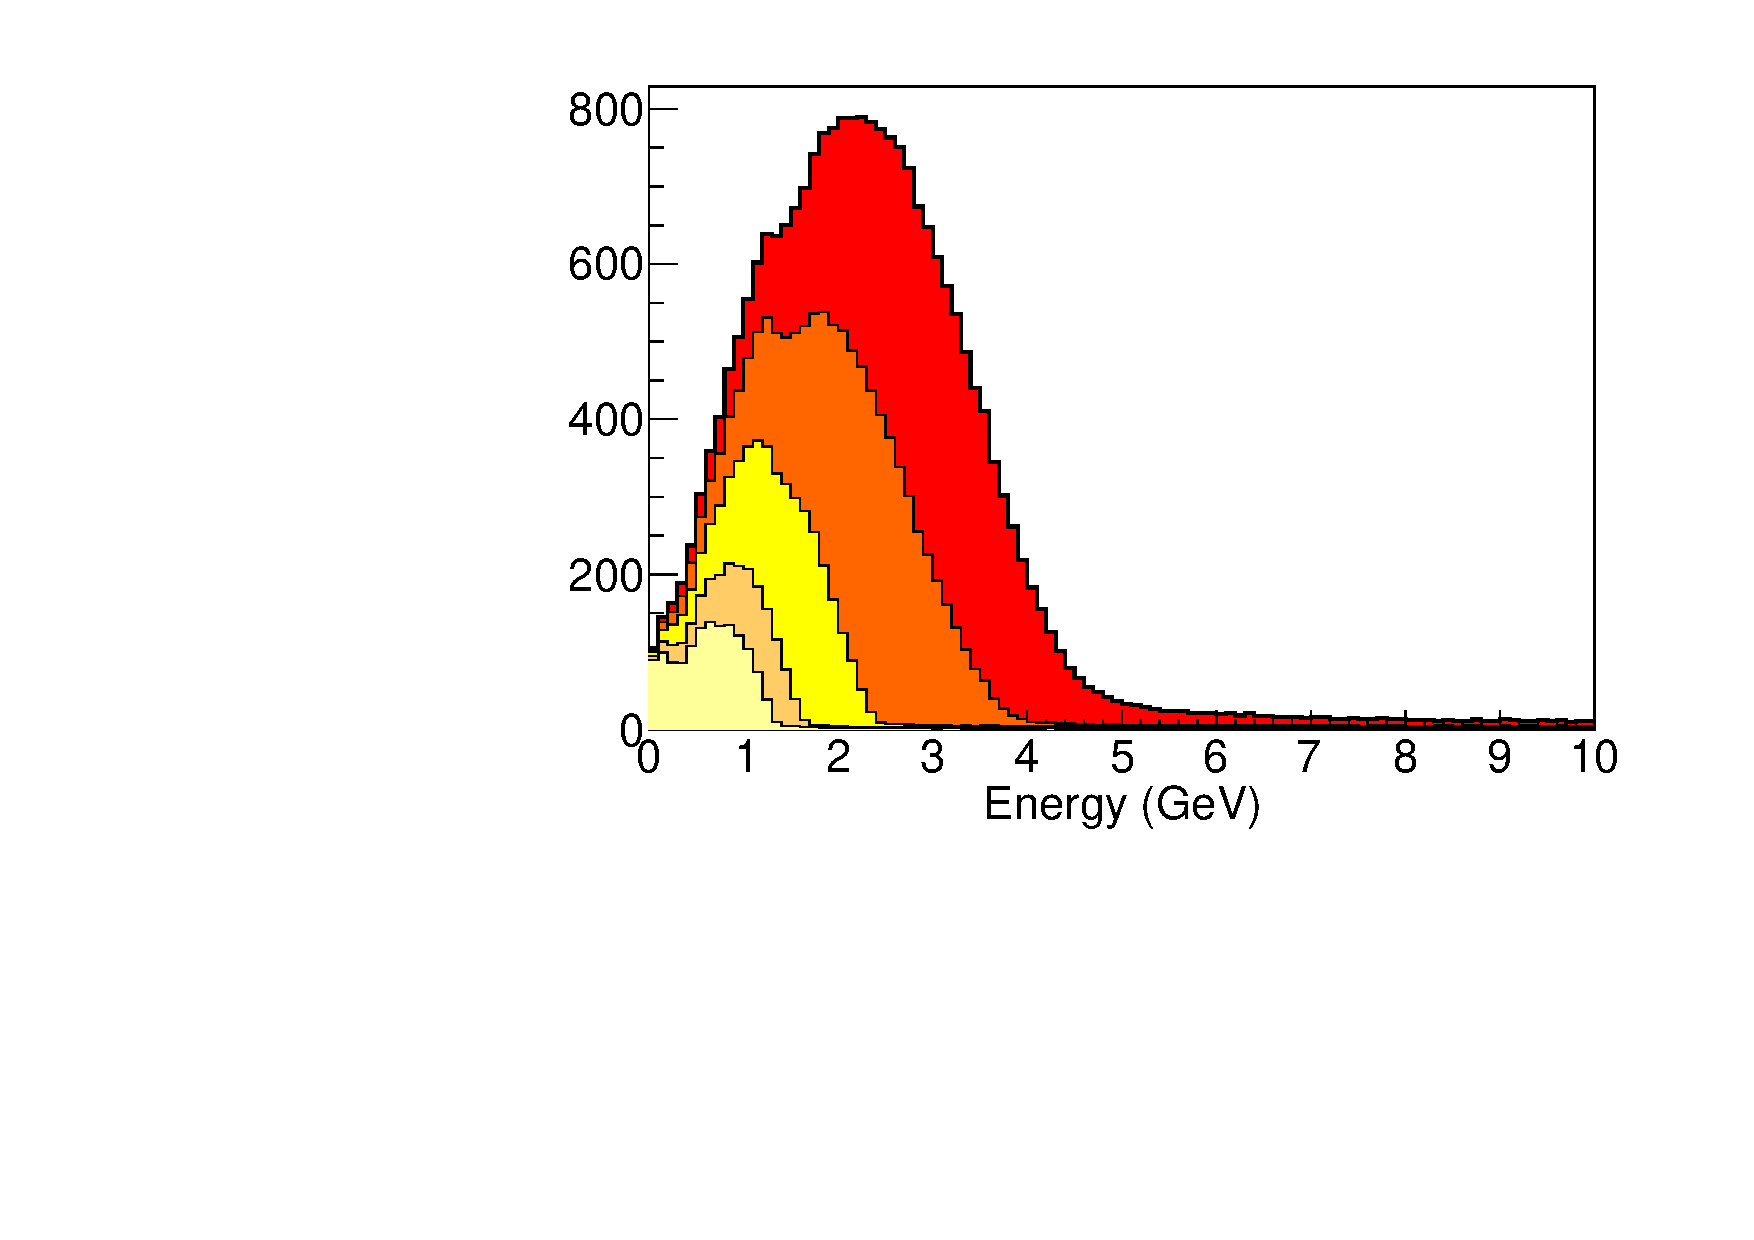
\includegraphics[width=0.5\linewidth]{Figures/DUNEbeam_truetimingB.pdf}
	\end{center}
	\caption{The DUNE forward horn current flux (red), with the
          fluxes corresponding to increasingly later time-cuts on the
          bunch time, assuming no time spread of the protons on
          target: 250 psec after the start of the neutrino bunch
          (orange), 500 psec after (yellow), 750 psec (dark beige), 1
          nsec (light beige).}
		\label{fig:Dunebeam_truetimingB}
\end{figure}


\begin{figure}[t]
	\begin{center}
           	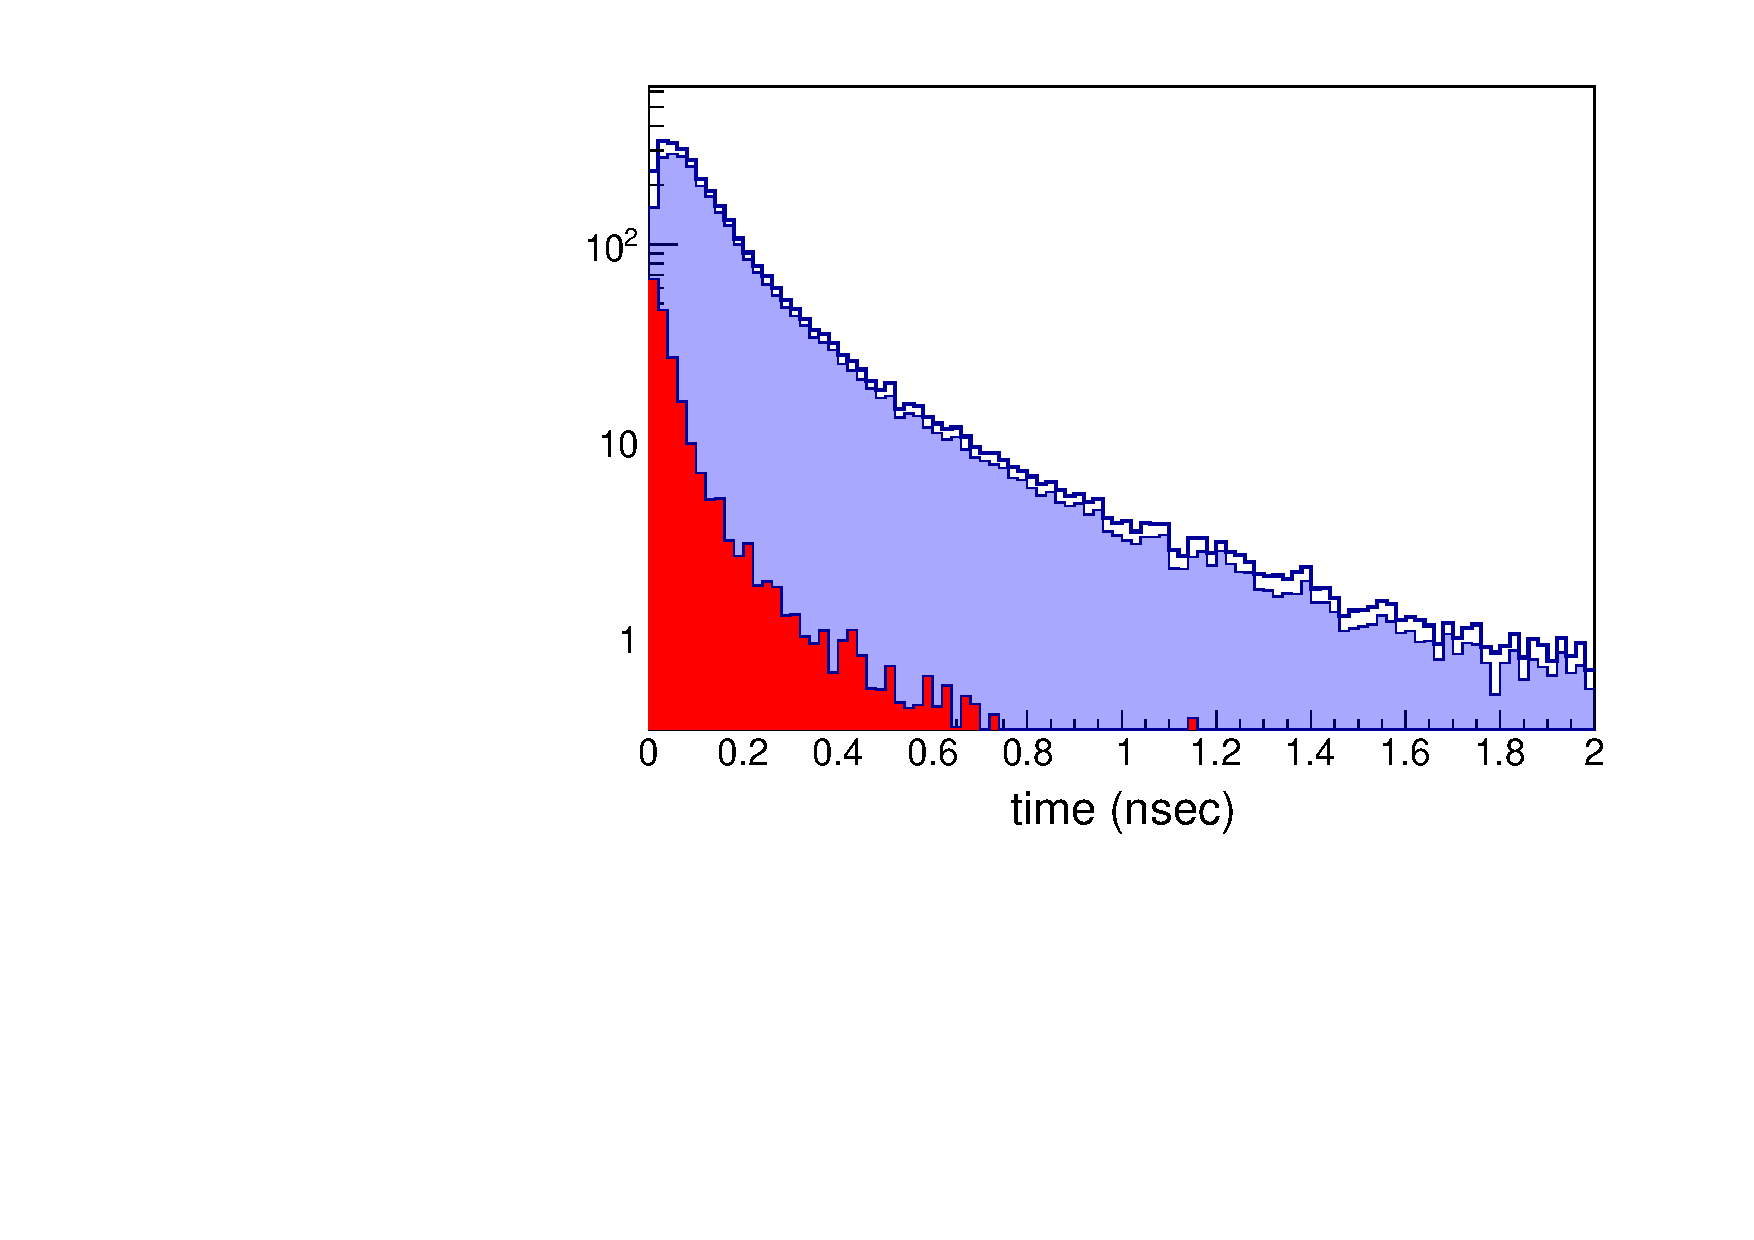
\includegraphics[width=0.5\linewidth]{Figures/RHCbeamcontent_log.pdf}
	\end{center}
	\caption{The time spectrum of anti-neutrinos in reverse horn
          current mode (blue) overlaid with wrong-sign neutrino
          contamination in red. The wrong-sign component drops off
          more quickly.}
		\label{fig:RHCbeamcontent_log}
\end{figure}

\subsection{Derivation of Time Dispersion}

The difference in arrival time of a neutrino from a sub-relativistic
pion of energy E' with respect to a high energy pion traveling with
speed $\sim$c is given by:

\begin{equation}
\Delta t(E') = \frac{c - v(E')}{c} \tau (E')
\end{equation}

Where $\tau (E')$ is the lifetime of the lower energy pion in the lab
frame. The time spreading will only occur until the decay of the lower
energy pion, at which point the daughter neutrinos will propagate at
c. The lifetime of the higher energy pion is irrelevant, since the
pion is already propagating at roughly c.

\begin{equation}
\Delta t(E') = \tau (E') [1 - \beta (E')]
\end{equation}

Rewriting in terms of the pion lifetime in the restframe, $\tau_0$, we get:

\begin{equation}
\Delta t(E') = \left(\frac{E'}{m} \tau_0\right) \left[1 - \sqrt{ 1 - \frac{m^2}{E'^2}} \right] 
\end{equation}

Regrouping the equation, we get the relationship:

\begin{equation}
\Delta t(E') = \left[\frac{E'}{m} - \sqrt{ \frac{E'^2}{m^2} - 1}\right] \tau_0
\label{eq:beamkinematicsandtiming}
\end{equation}

As one would expect, at the lowest energies, where the pion is
essentially at rest in the lab frame, $\Delta t(E')$ approaches the
lifetime of the pion in the rest frame, $\tau_0$. At high energies,
the speed of the lower-energy pion approaches that of the higher
energy pion and thus $\Delta t(E')$ goes to zero.

Figure~\ref{fig:beamkinematicsandtiming} shows a plot of
equation~\ref{eq:beamkinematicsandtiming} (TOP), and the simulated
relationship between $\Delta t(E')$ and E' for the DUNE beam.

\begin{figure}[h]
	\begin{center}
           	\begin{tabular}{c c}
 \multicolumn{2}{c}{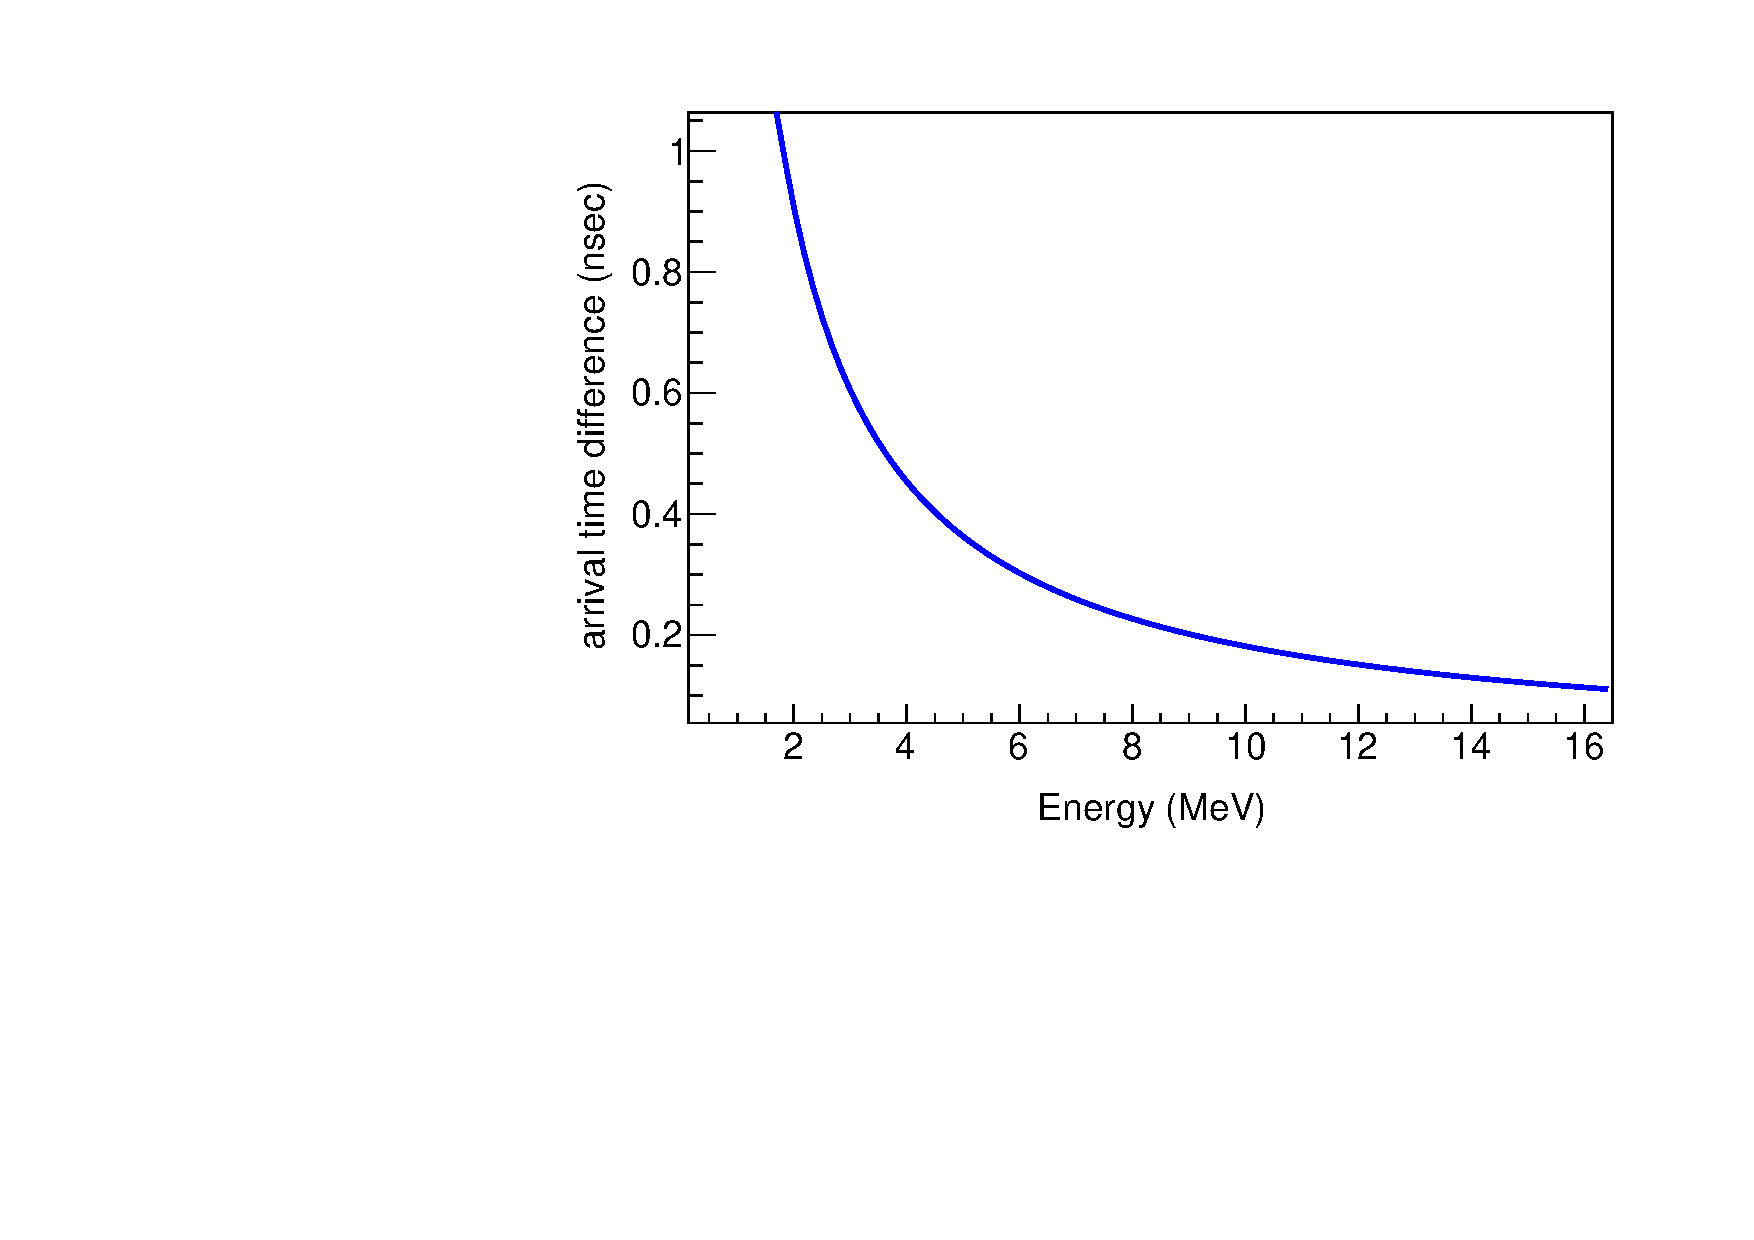
\includegraphics[width=0.5\linewidth]{Figures/deltaTvsE.pdf}} \\
 \includegraphics[width=0.49\linewidth]{Figures/parentEvsdT.pdf} &
 \includegraphics[width=0.49\linewidth]{Figures/nuEvsdT.pdf} \\
			\end{tabular}
%           	\begin{tabular}{c c}
%           	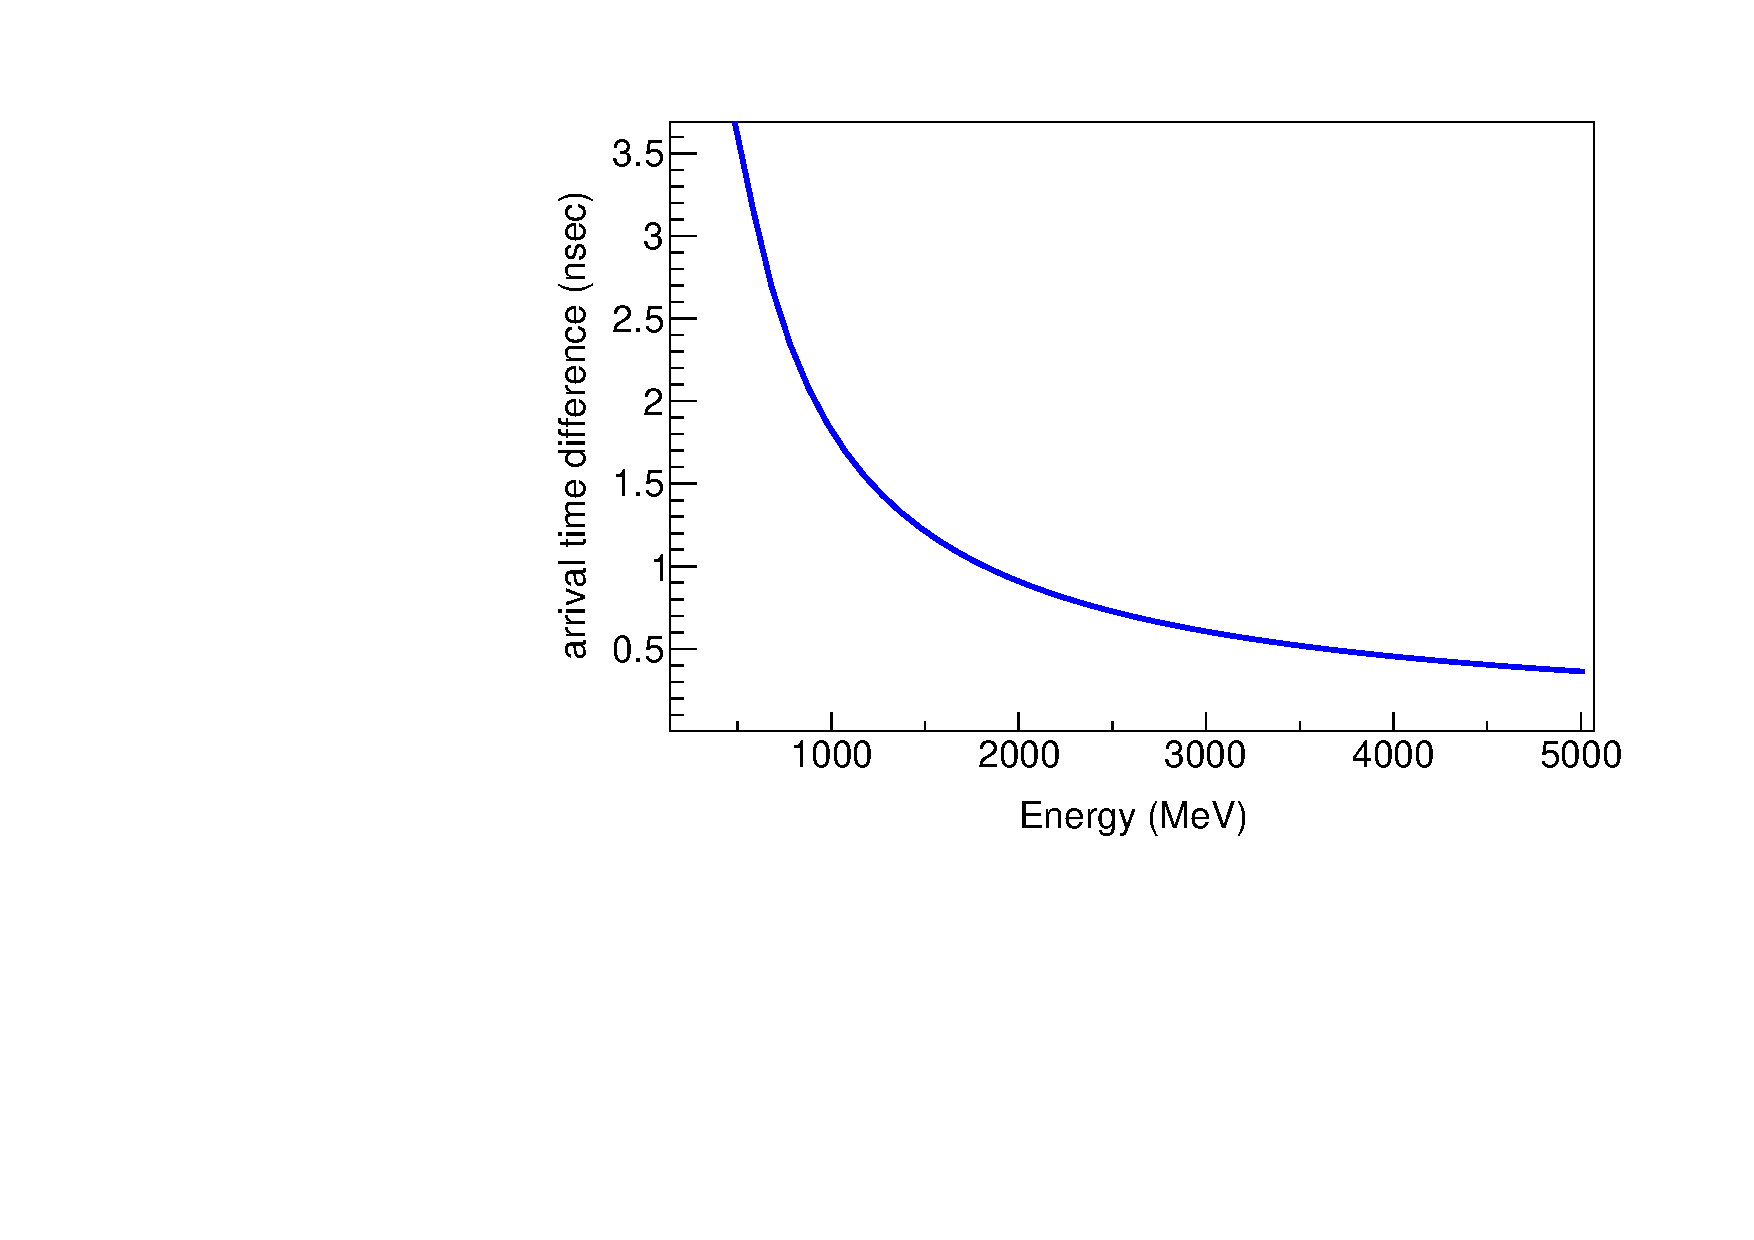
\includegraphics[width=0.455
%                  \linewidth]{Figures/2018.12.3_kinematics/deltaTvsE.pdf}
%                & \includegraphics[width=0.49
%                  \linewidth]{Figures/2018.10.14_LBNFtiming/parentEvsdT.pdf}
%                \\ \multicolumn{2}{c}{\includegraphics[width=0.5
%                    \linewidth]{Figures/2018.10.14_LBNFtiming/nuEvsdT.pdf}}
%			\end{tabular}
	\end{center}
	\caption{Top: A plot of the peak time difference between the arrival of neutrinos from a sub-relativistic pion of energy E' with respect to a relativistic pion (Eq~\ref{eq:beamkinematicsandtiming}). Bottom Left: The simulated relationship between the arrival times and pion energies, for a population of pions produced at the same time. Bottom Right: The equivalents plot of arrival time difference for different energies of the neutrinos.}
		\label{fig:beamkinematicsandtiming}
\end{figure}


\subsection{Impact of Bunch Size}
\label{bunch_size}

Just showing that wider bunches wash out the effect (short section)


%\begin{figure}[t]
%	\begin{center}
%           	\begin{tabular}{c c}	
%           	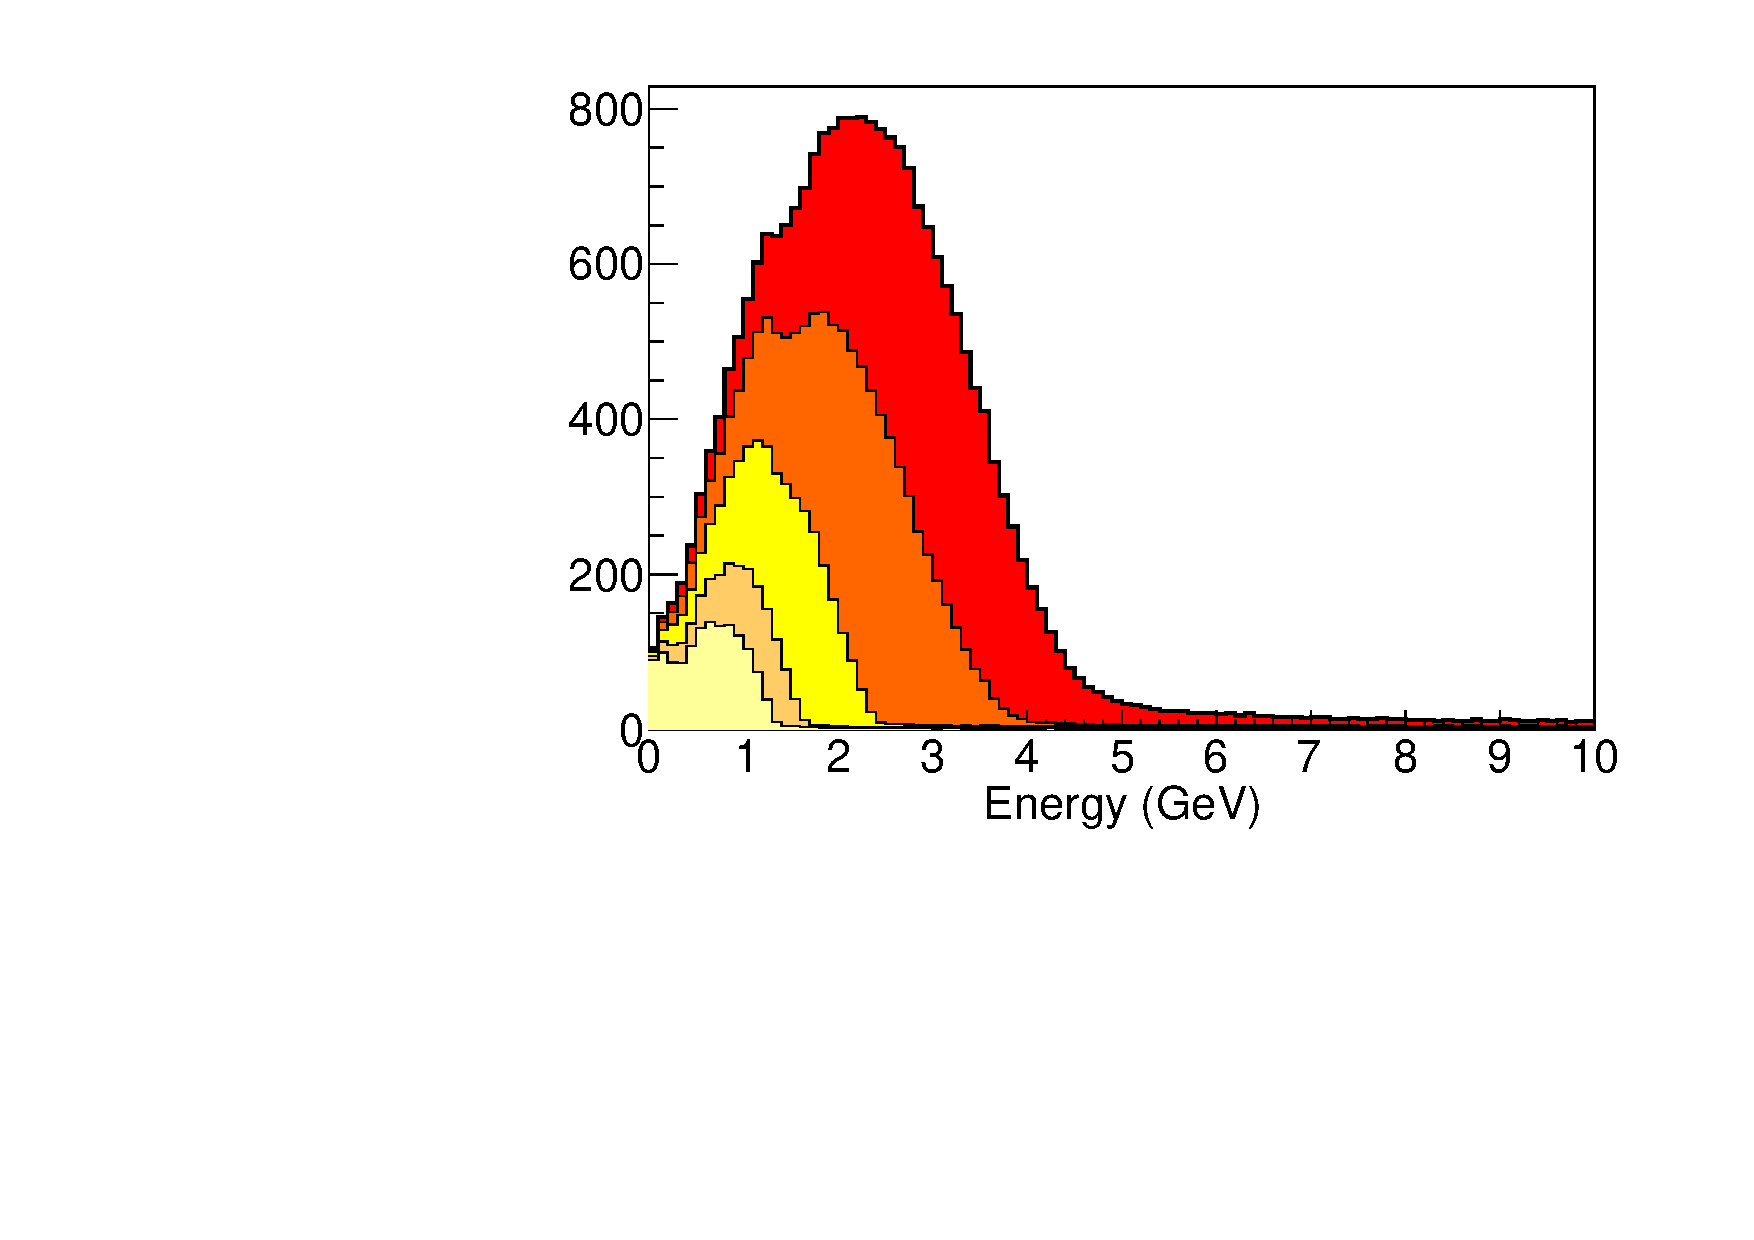
\includegraphics[width=0.49
%                  \linewidth]{Figures/DUNEbeam_truetimingB.pdf}
%                & 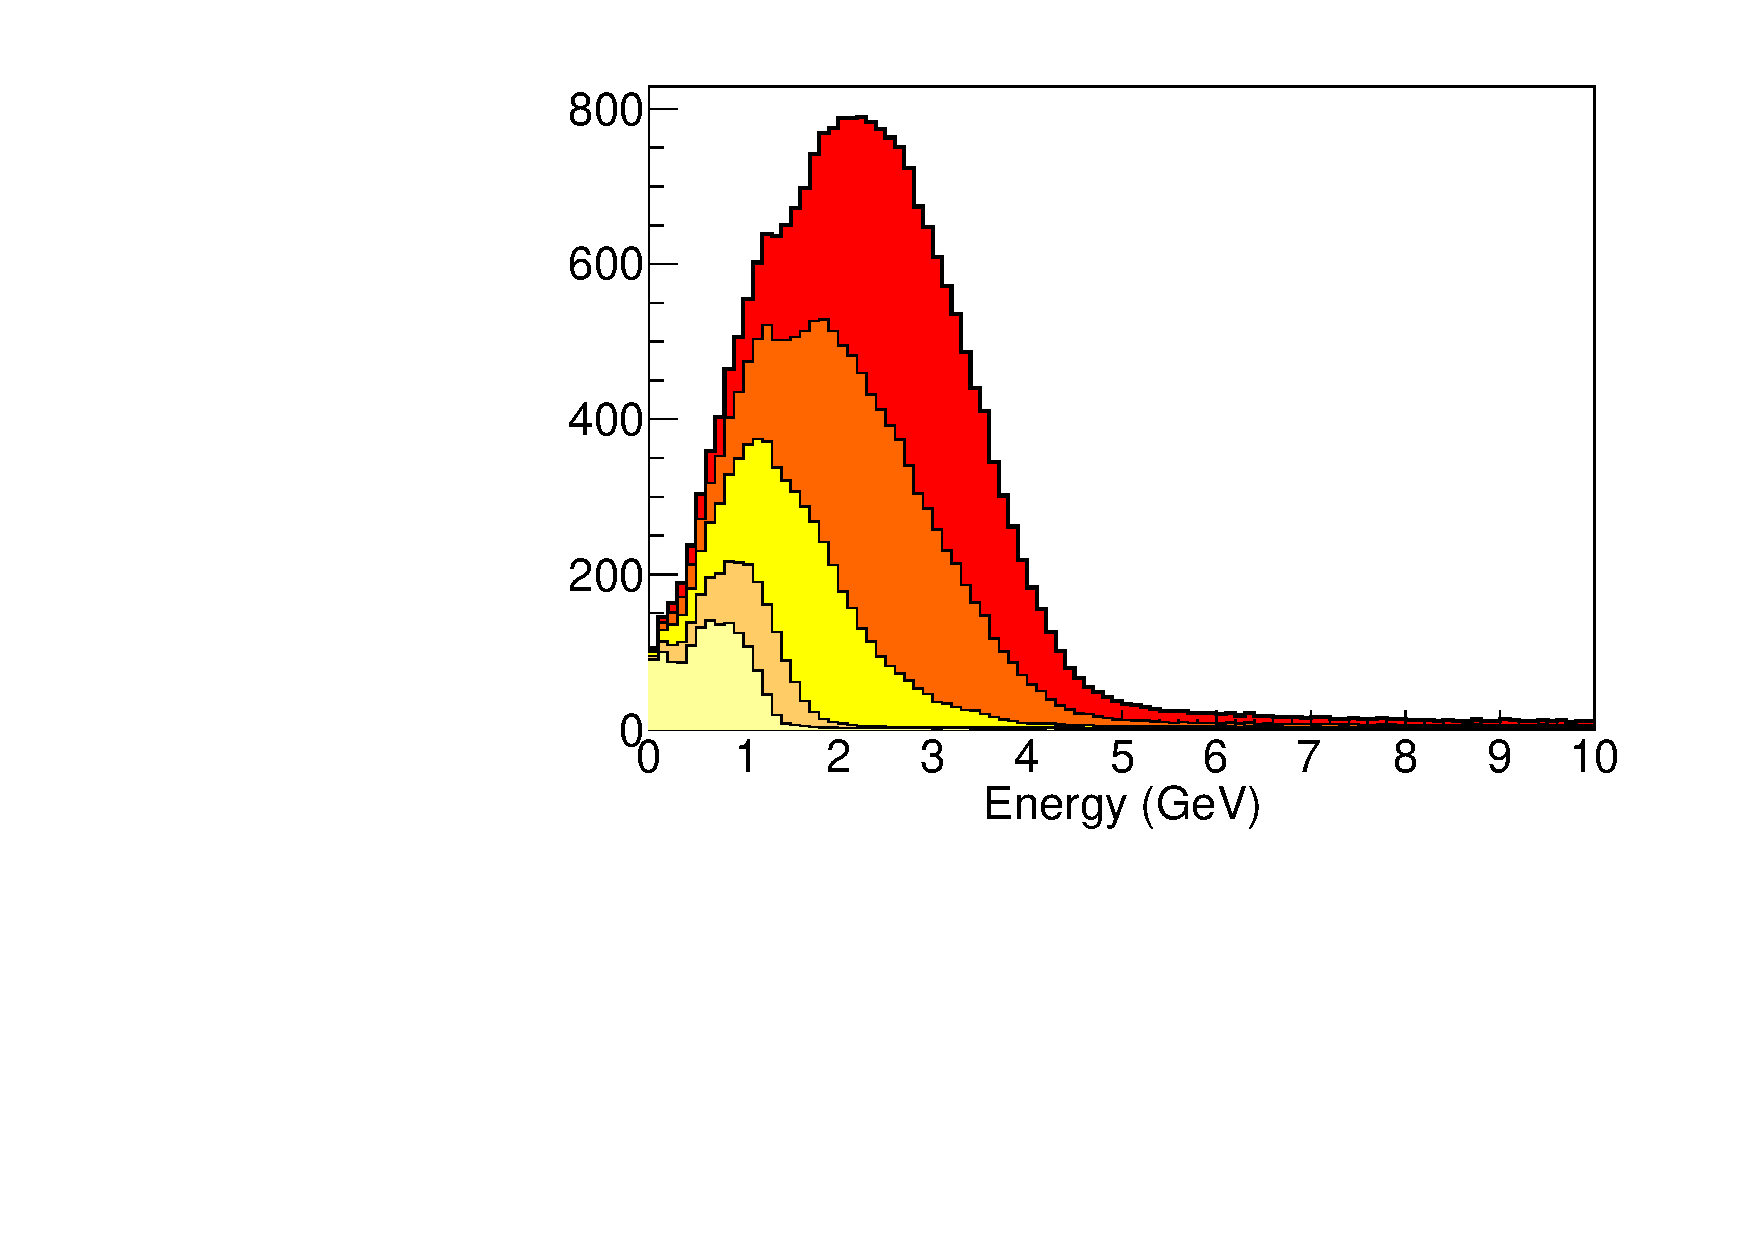
\includegraphics[width=0.49
%                  \linewidth]{Figures/DUNEbeam_100psecB.pdf}
%                \\ 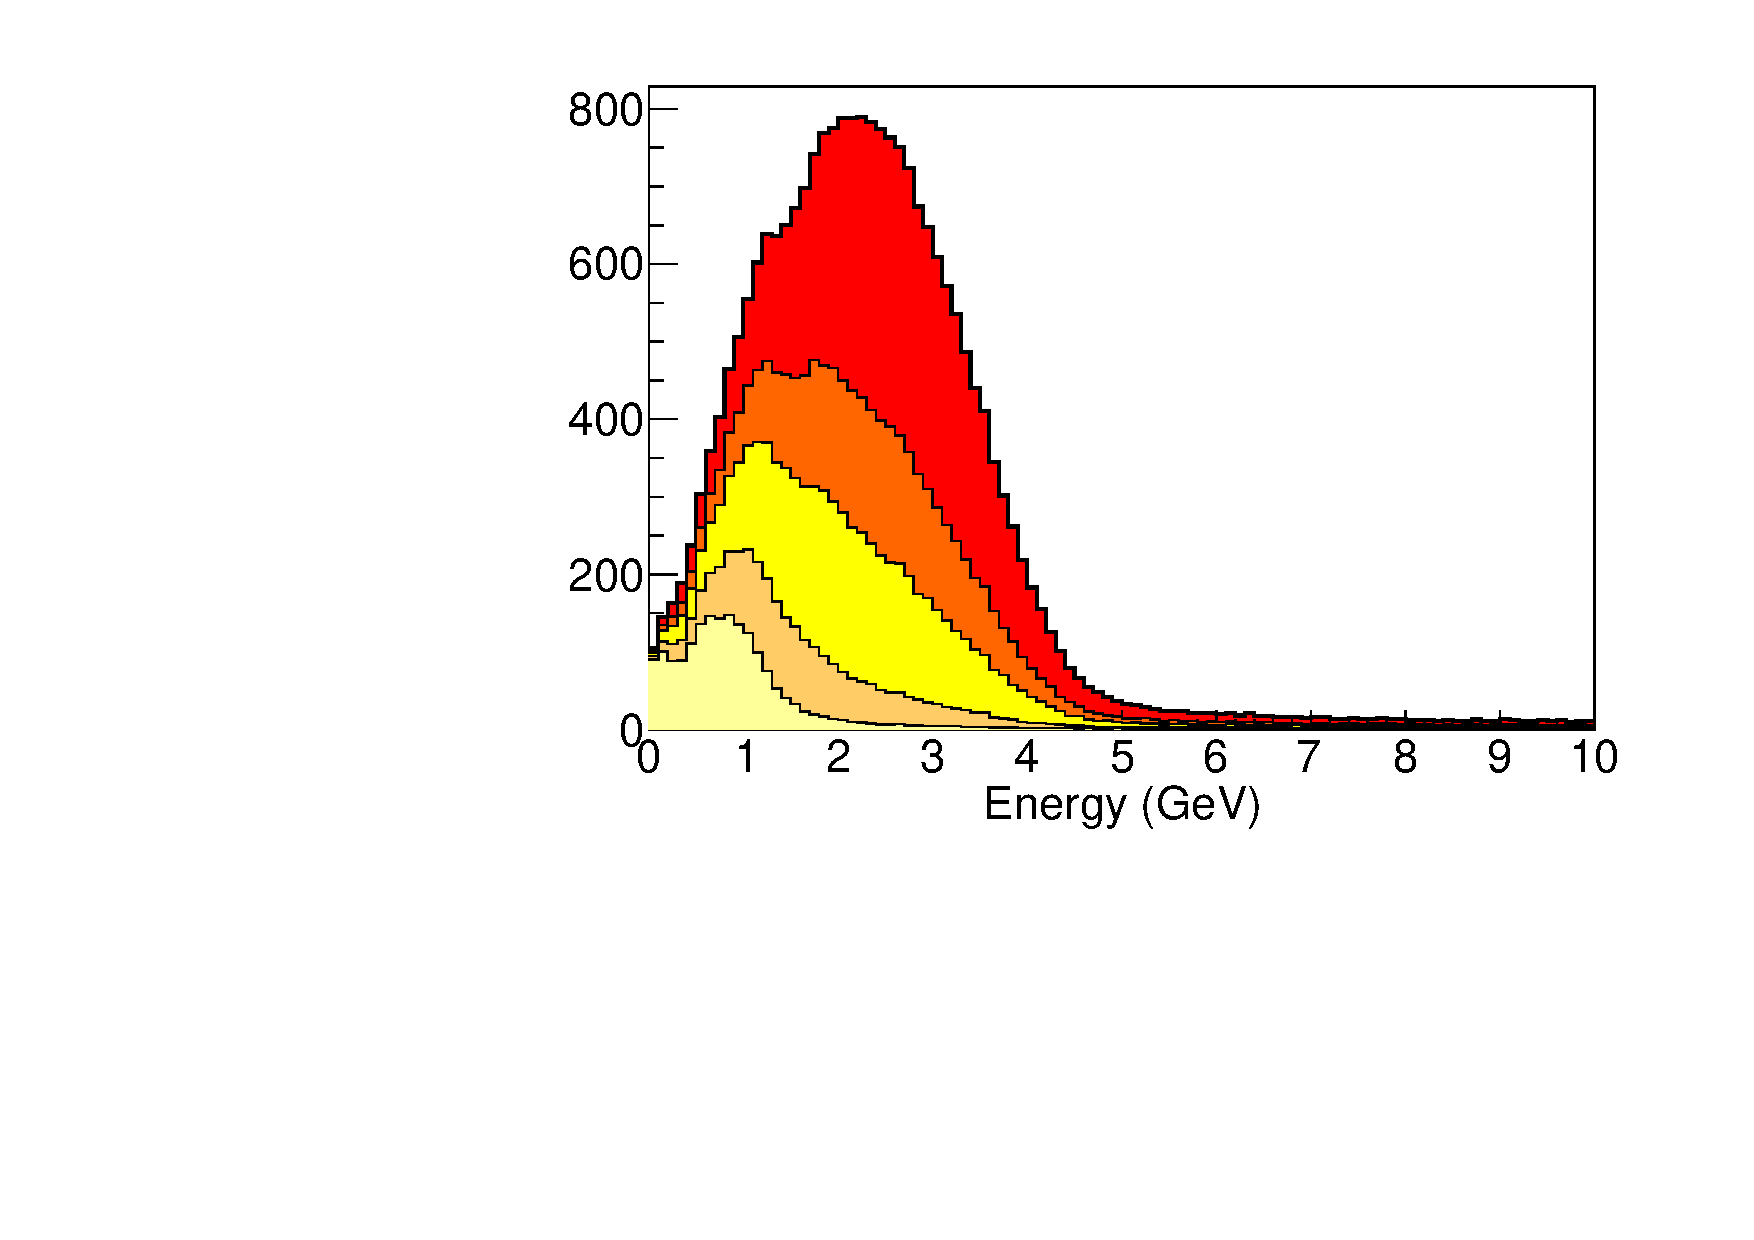
\includegraphics[width=0.49
%                  \linewidth]{Figures/DUNEbeam_250psecB.pdf}
%                & 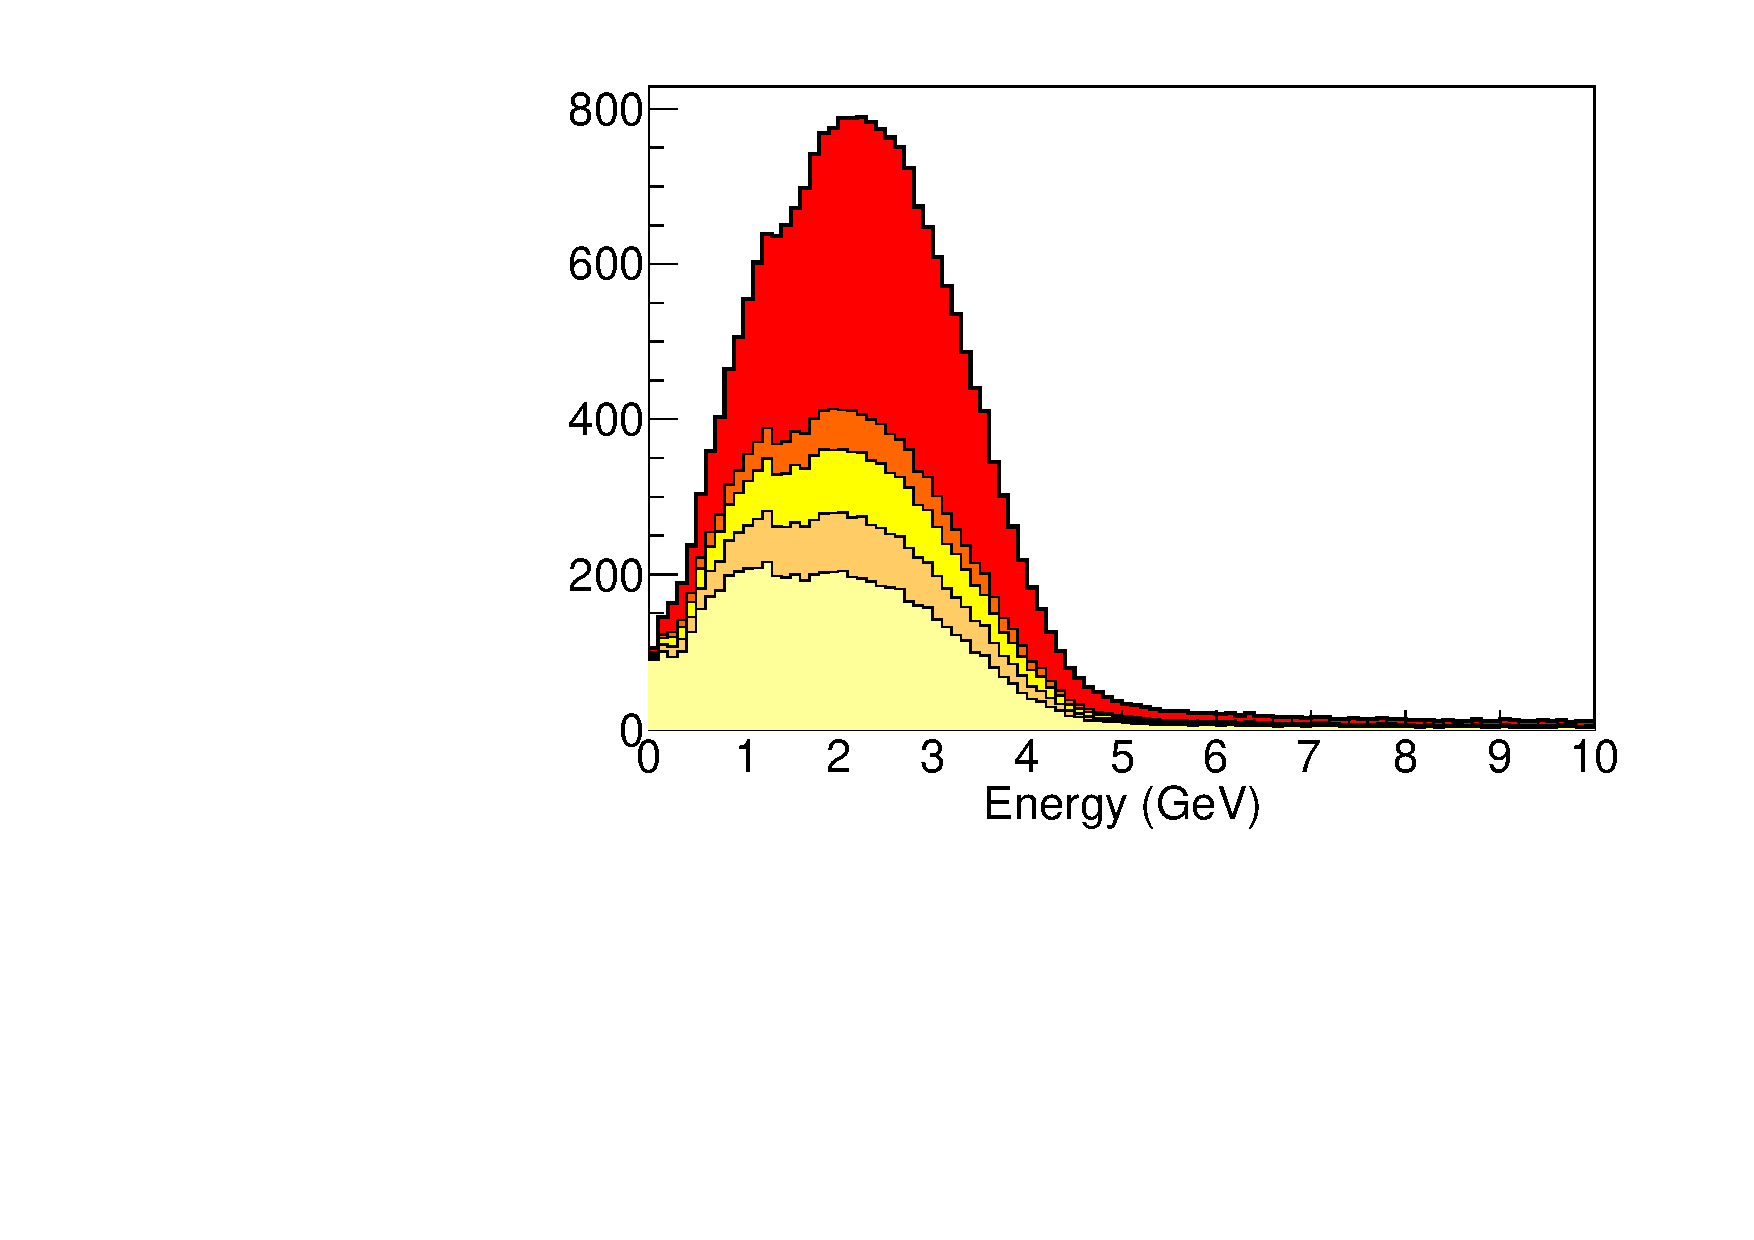
\includegraphics[width=0.49
%                  \linewidth]{Figures/DUNEbeam_900psecB.pdf}
%                \\
%			\end{tabular}
%	\end{center}
%	\caption{A series of panels showing the DUNE forward horn current flux (red), overlaid with the fluxes corresponding to increasingly later time-cuts on the bunch time, assuming no time spread of the protons on target: 250 psec after the start of the neutrino bunch (orange), 500 psec after (yellow), 750 psec (dark beige), 1 nsec (light beige). The UPPER LEFT panel corresponds to a case where all protons hit the target instantaneously. The UPPER RIGHT panel corresponds to a proton bunch with 100 psec width. The LOWER left panel corresponds to a 250 psec bunch width and the LOWER RIGT corresponds to 900 psec.}
%		\label{fig:anniedetector}
%\end{figure}


% End of Section 4
